%Template 2: Star Wars!
\begin{titlepage}



\pagestyle{empty}
% Begin tikz picture, remember the picture
\begin{tikzpicture}[overlay,remember picture]


%Shaded Arcs
\node[circle, minimum size=20cm, fill=gray!15] at (0,-15) {};
\node[circle, minimum size=14cm, fill=yellow!20] at (16,-7) {};
\node[circle, minimum size=10cm, fill=orange!10] at (16,-21) {};


% Node(s) 1: Death Star
\newcommand{\baseSTARX}{14}
\newcommand{\baseSTARY}{-2}
\newcommand{\baseSTARR}{3.5}
\newcommand{\baseDISCX}{\baseSTARX - 1}
\newcommand{\baseDISCY}{\baseSTARY - 0.3}
\newcommand{\baseDISCR}{1}
\newcommand{\baseDISCRH}{\baseDISCR*0.70710678118}
\newcommand{\distanceBetweenHorizontalLines}{20}

%Nodes describing base shape
\node[circle, minimum size=7cm, draw=black, fill=lightgray] at (\baseSTARX,\baseSTARY) {};

%Command takes input: degree, radius, centerX, centerY
% Turns out sine and cosine take angles.... (probably should have known this)
\newcommand{\calchorizontal}[4]{
({(#3) - (#2) * cos((#1))},
{(#4) + (#2) * sin((#1))}) 
-- 
({(#3) + (#2) * cos((#1))},
{(#4) + (#2) * sin((#1))})
}
% Command takes inputs degree, radius, centerX, centerY, d(lines), height
\newcommand{\calcvertical}[6]{
({(#3) - (#2) * cos((#1)) + (#6)},
{(#4) + (#2) * sin((#1))}) 
-- 
({(#3) - (#2) * cos((#1)) + (#6)},
{(#4) + (#2) * sin((#1)) + (#5)})
}

% Takes input radius, n
\newcommand{\calcVerticalDistance}[2]{
2*(#1)*sin(0.5*(\distanceBetweenHorizontalLines))*cos(0.5*(2*(#2)+1)*(\distanceBetweenHorizontalLines))
}


\def\lineARRAYA{{-0.3, 1.1, 5, 6.2,2,4,1.6,1.7,1.8}}
\def\lineARRAYB{{1, 1.6, 1.2, 1.3,5.3,1.5,1.6,1.7,-1.8}}

\foreach \n in {-4,...,4}{
%nodes describing various compartments
\draw [black, line width=1] \calchorizontal{\n * \distanceBetweenHorizontalLines}{\baseSTARR}{\baseSTARX}{\baseSTARY};

\draw [black, line width=1] \calcvertical{\n * \distanceBetweenHorizontalLines}{\baseSTARR}{\baseSTARX}{\baseSTARY}{\calcVerticalDistance{\baseSTARR}{\n}}{\lineARRAYA[\n+4]};
\draw [black, line width=1] \calcvertical{\n * \distanceBetweenHorizontalLines}{\baseSTARR}{\baseSTARX}{\baseSTARY}{\calcVerticalDistance{\baseSTARR}{\n}}{\lineARRAYB[\n+4]};


}





% TODO SCORESH: MAKE THIS WORK PLEASE <3       ==> ISSUES WITH FORMATTING, NEED TO CHECK IF, THEN
%\pgfmathsetseed{14} 
% \foreach \n in {-4,...,4}{
% % generate random n
% \pgfmathrandominteger{\rand}{0}{100}
% % --------------- FIRST SET -------------


% \draw [black, line width=1]
% \calcvertical{
% \n * \distanceBetweenHorizontalLines}{
% \baseSTARR}{
% \baseSTARX}{
% \baseSTARY}{
% \calcVerticalDistance{\baseSTARR}{\n}}{\rand};

% % generate random n
% \pgfmathrandominteger{\rand}{0}{100}
% % --------------- SECOND SET -------------


% \draw [black, line width=1]
% \calcvertical{
% \n * \distanceBetweenHorizontalLines}{
% \baseSTARR}{
% \baseSTARX}{
% \baseSTARY}{
% \calcVerticalDistance{\baseSTARR}{\n}}{\rand};
% }


%Disc for laser
\node[circle, minimum size=2cm, draw=black, fill=gray] at (\baseDISCX,\baseDISCY) {};
\node[circle, minimum size=1.5cm, draw=black, fill=gray] at (\baseDISCX,\baseDISCY) {};




% Node 3 setup (Alderran)
\newcommand{\basePLANETX}{1}
\newcommand{\basePLANETY}{-4}



%Node(s) 2: Laser
\newcommand{\baseFOCIX}{7}
\newcommand{\baseFOCIY}{-3}
\newcommand{\baseLASERW}{2.5}

%center
\draw [green, line width=\baseLASERW-1] (\baseFOCIX,\baseFOCIY) -- (\baseDISCX,\baseDISCY);

%modX
\draw [green, line width=\baseLASERW] (\baseFOCIX,\baseFOCIY) -- (\baseDISCX + \baseDISCR,\baseDISCY);
\draw [green, line width=\baseLASERW] (\baseFOCIX,\baseFOCIY) -- (\baseDISCX - \baseDISCR,\baseDISCY);

%modY
\draw [green, line width=\baseLASERW] (\baseFOCIX,\baseFOCIY) -- (\baseDISCX,\baseDISCY + \baseDISCR);
\draw [green, line width=\baseLASERW] (\baseFOCIX,\baseFOCIY) -- (\baseDISCX,\baseDISCY - \baseDISCR);

%modDiagonals
\draw [green, line width=\baseLASERW] (\baseFOCIX,\baseFOCIY) -- (\baseDISCX + \baseDISCRH,\baseDISCY + \baseDISCRH);
\draw [green, line width=\baseLASERW] (\baseFOCIX,\baseFOCIY) -- (\baseDISCX + + \baseDISCRH,\baseDISCY - \baseDISCRH);


%laser to planet
\draw [green, line width=\baseLASERW] (\baseFOCIX,\baseFOCIY) -- (\basePLANETX, \basePLANETY);


% Node(s) 3: Alderran
\node (planet) at (\basePLANETX,\basePLANETY) {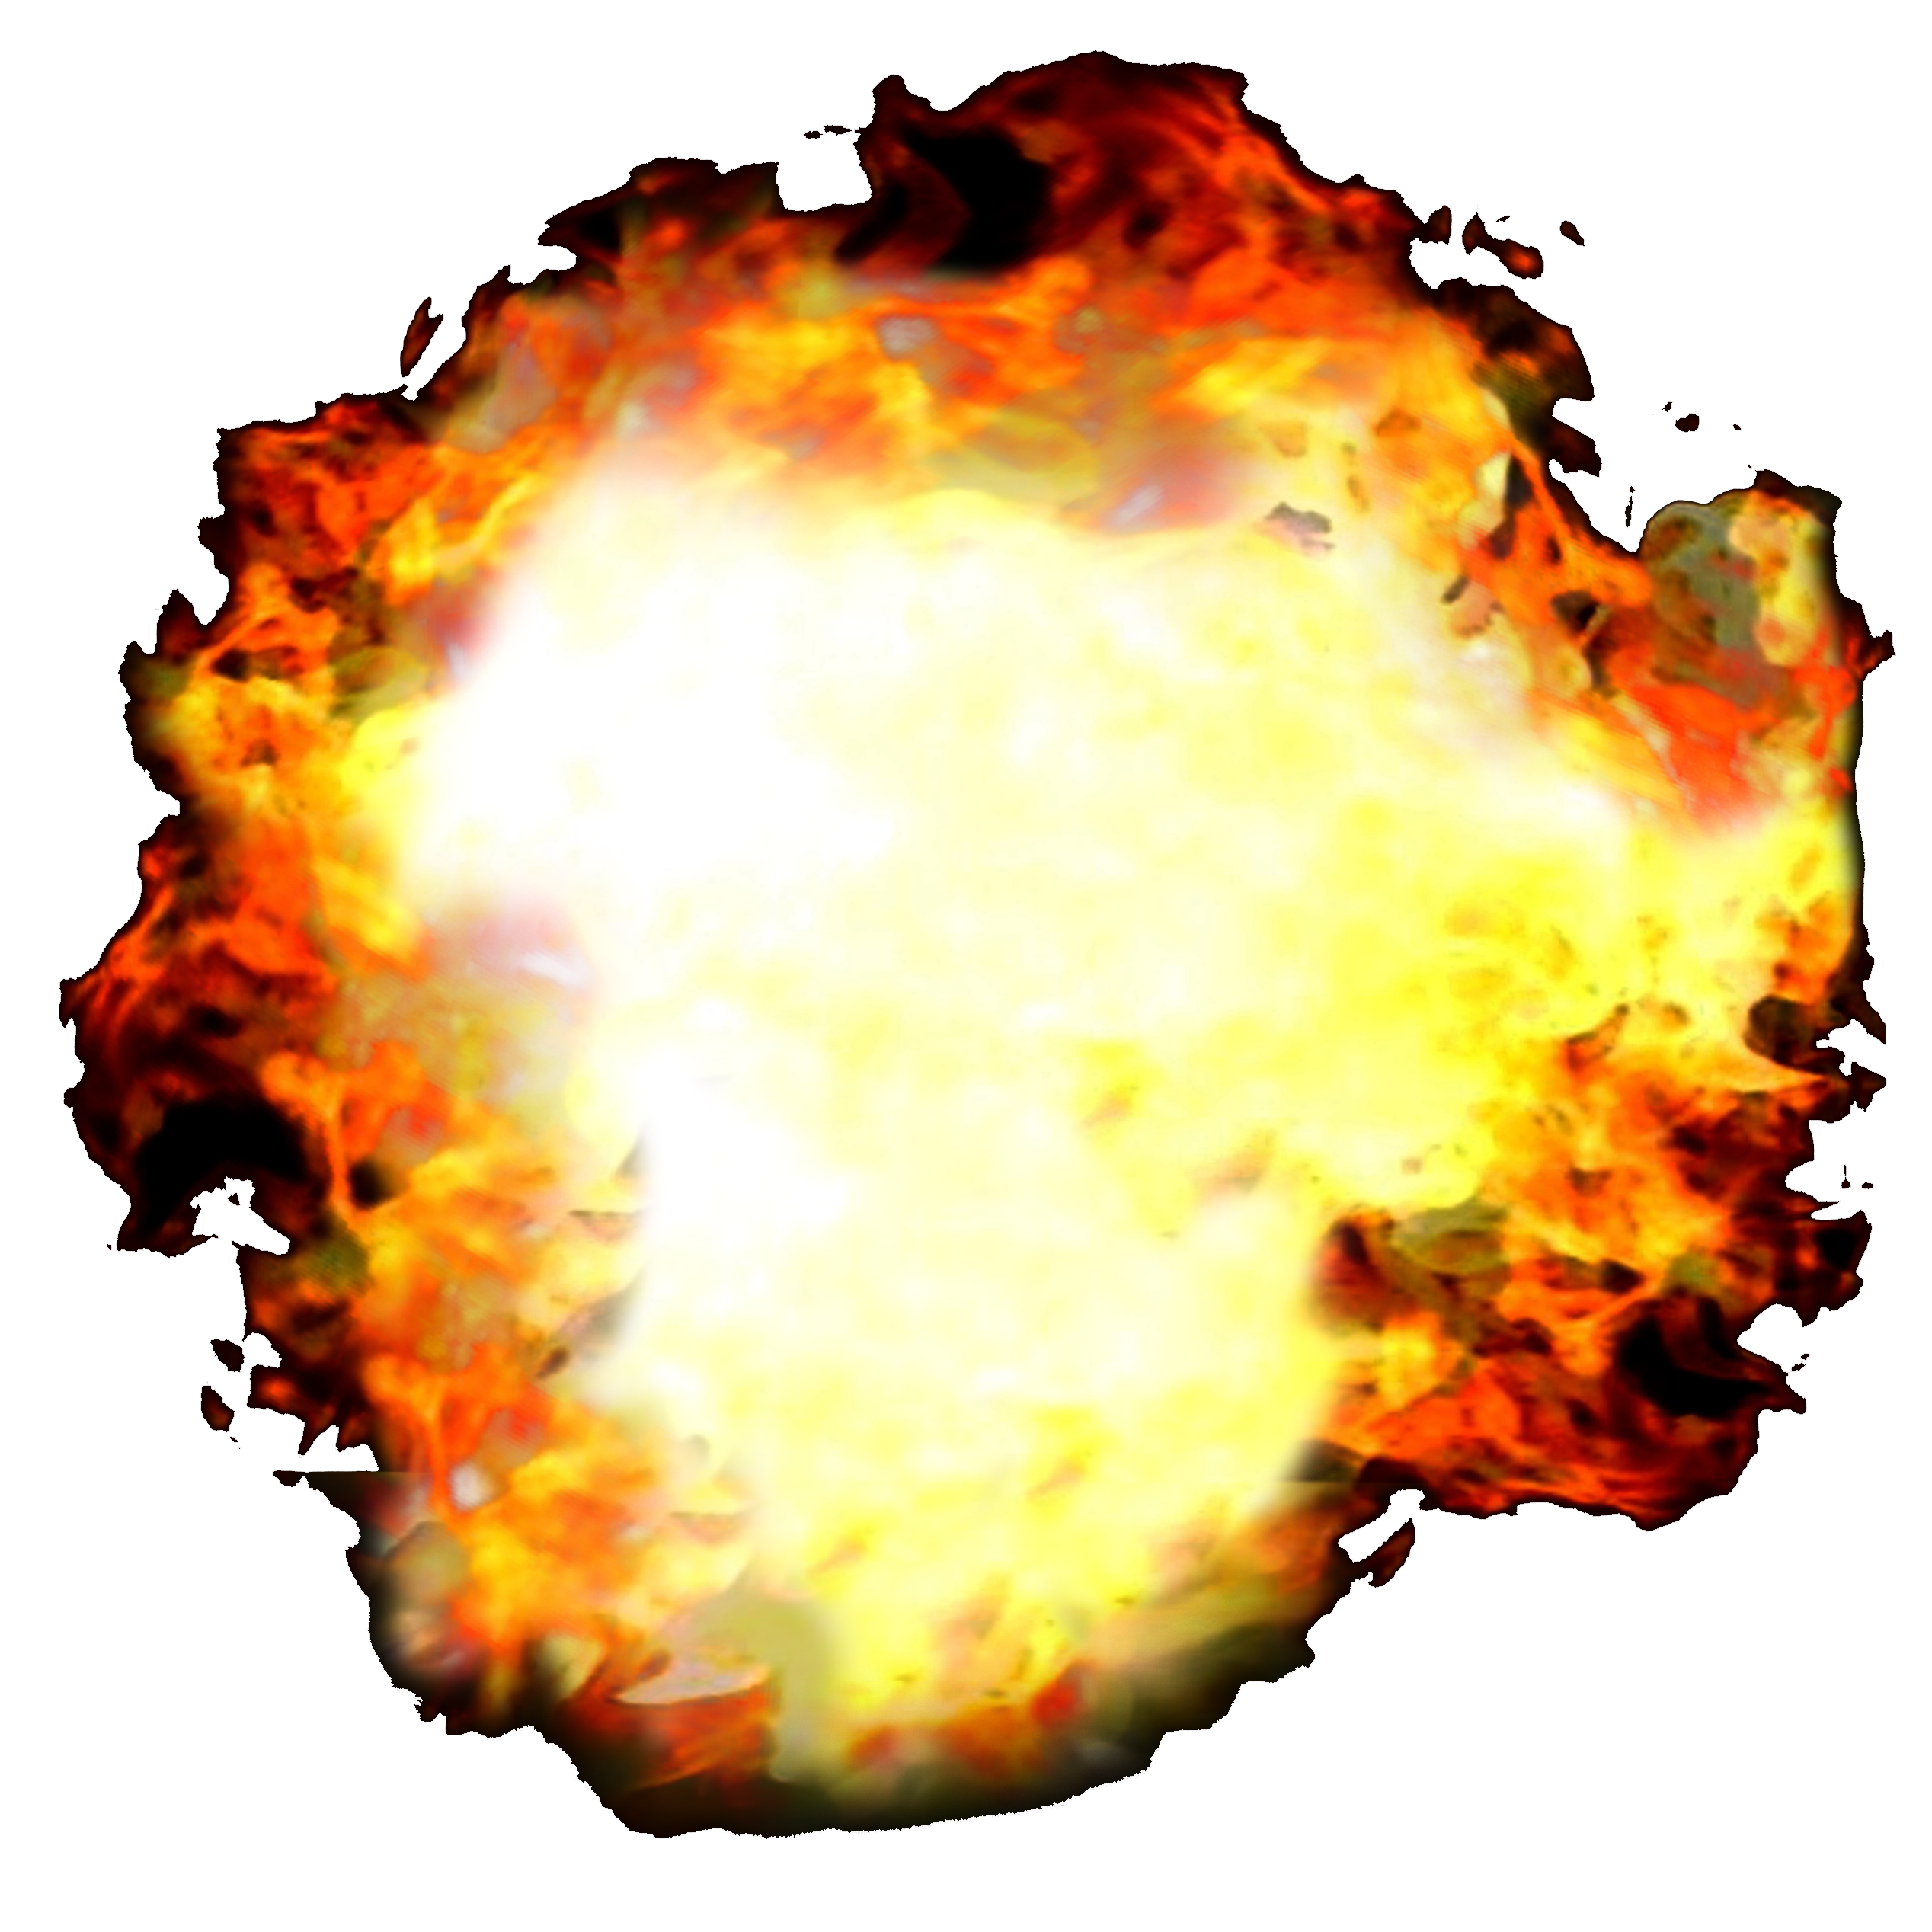
\includegraphics[width=3.5cm]{images/expEDITED.png}};
\node (planet) at (\basePLANETX,\basePLANETY) {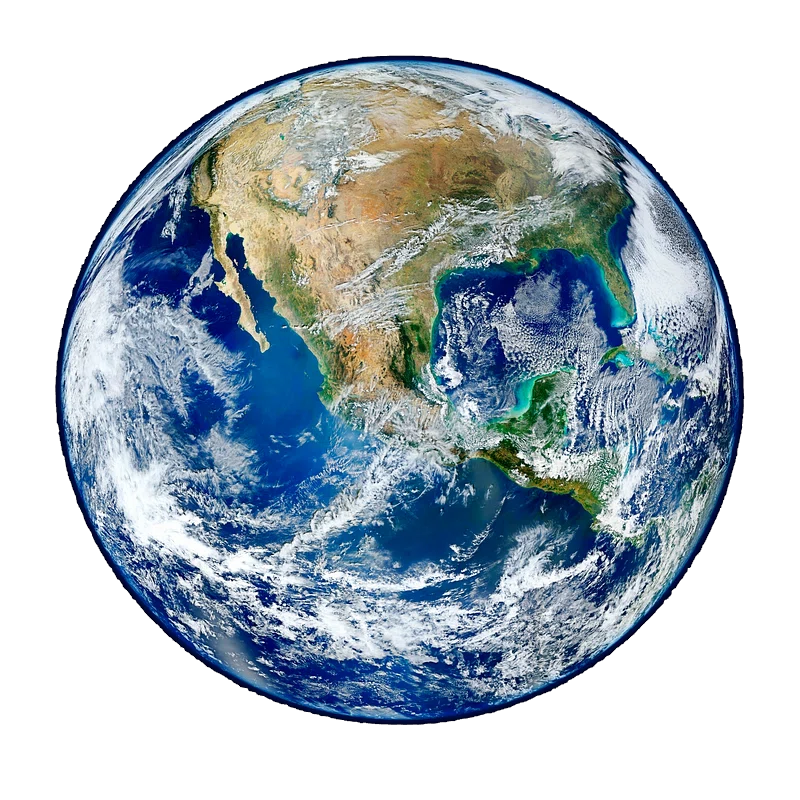
\includegraphics[width=3cm]{images/earthEDITED.png}};






% END GRAPHICS



% TITLE, AUTHOR, CLASS, DATE
\node[
align=center
]
at ($(current page.center)+(0,2)$) {
    \fontsize{60}{72} \selectfont \textcolor{black}{\titleDOC}
    \\[6pt] \fontsize{16}{19.2} \selectfont \textcolor{red}{ \bf \authorDOC} 
    \\[6pt] \classDOC \\[6pt] \dateDOC
};



% QUOTE (above laser)
\node[text width=9.5cm,
      align=center,
      rotate={atan((\baseSTARY-\basePLANETY)/(\baseSTARX-\basePLANETX))}      
] at (\baseFOCIX-0.75,\baseFOCIY+1) { 
\fontsize{12}{13.2} \selectfont \quoteDOC
};


% \node[text width=1.1in,align=center] at ($(current page.center)+(8.5,-13)$) {{
%     Generated by Scoresh's Lab-Gen
% }};

\node[anchor=north west, %anchor is upper left corner of the graphic
      xshift=6.7in, %shifting around
      yshift=-9in] 
     at (current page.north west) %left upper corner of the page
     {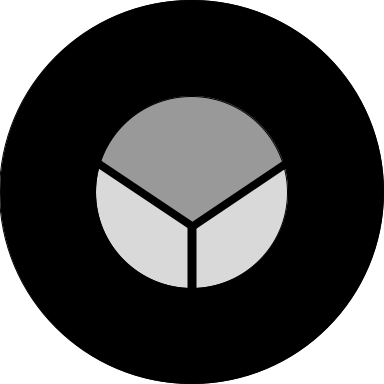
\includegraphics[width=1.5in]{images/labgen_logo.png}}; 

\node[anchor=north west, %anchor is upper left corner of the graphic
      xshift=0.3in, %shifting around
      yshift=-9in] 
     at (current page.north west) %left upper corner of the page
     {
\includegraphics[width=1.5in]{images/portsmouth_logo.png}}; 





\end{tikzpicture}

% \begin{figure}[htbp]
%     \centering
%     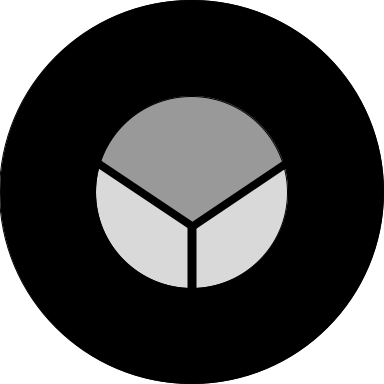
\includegraphics[width=0.3\textwidth]{images/labgenpng.png}
% \end{figure}



\end{titlepage}
